\documentclass[12pt,a4paper]{report}
\usepackage[utf8]{inputenc}
\usepackage[T5]{fontenc} % Tiếng Việt
\usepackage{graphicx}
\usepackage{float}
\usepackage[hidelinks]{hyperref} % Xóa viền đỏ mục lục
\usepackage{geometry}
\usepackage{array}
\usepackage{tabularx}
\usepackage{amsmath}
\geometry{a4paper, margin=1in}
\usepackage{listings}
\usepackage{xcolor}
\usepackage{tikz}
\lstdefinestyle{sqlstyle}{
    language=SQL,
    backgroundcolor=\color{gray!5},
    basicstyle=\ttfamily\footnotesize,
    keywordstyle=\color{blue}\bfseries,
    stringstyle=\color{red},
    commentstyle=\color{green!60!black},
    numbers=left,
    numberstyle=\tiny\color{gray},
    stepnumber=1,
    breaklines=true,
    frame=single,
    showstringspaces=false
}
\renewcommand{\tablename}{Bảng}
\renewcommand{\contentsname}{MỤC LỤC}

% Gói vẽ sơ đồ
\usepackage{tikz}
\usetikzlibrary{shapes.geometric, arrows.meta, positioning, automata}
\renewcommand{\chaptername}{Chương}
\renewcommand{\figurename}{Hình}
\renewcommand{\tablename}{Bảng}
\renewcommand{\contentsname}{Mục lục}
\begin{document}

% ================= TRANG BÌA =================
\begin{titlepage}
    \centering
    \vspace*{1cm}
    
    {\fontsize{14pt}{1cm}\selectfont \textbf{TRƯỜNG ĐẠI HỌC GIAO THÔNG VẬN TẢI}} \\
    {\fontsize{14pt}{1cm}\selectfont \textbf{PHÂN HIỆU TẠI TP. HỒ CHÍ MINH}} \\
    \vspace{1cm}
    
    % Nếu có logo trường, bỏ dấu % ở 2 dòng dưới và cho file logo.png vào thư mục images
    % \includegraphics[width=4cm]{images/logo.png} \\
    % \vspace{1cm}
    
    {\fontsize{20pt}{1cm}\selectfont \textbf{BÁO CÁO BÀI TẬP LỚN}} \\
    \vspace{0.5cm}
    {\fontsize{16pt}{1cm}\selectfont \textbf{MÔN: THIẾT KẾ CƠ SỞ DỮ LIỆU}} \\
    \vspace{2.5cm}
    
    {\fontsize{16pt}{1cm}\selectfont \textbf{Đề tài: Thiết kế Cơ sở Dữ liệu cho Nền tảng Dịch vụ Tín dụng \& Điểm thưởng cấp doanh nghiệp (OctaPoint CaaS)}} \\
    
    \vspace{4cm}
    
    \begin{center}
        \large
        \textbf{Nhóm sinh viên thực hiện:}\\[0.5cm]
        \renewcommand{\arraystretch}{1.3} % Tăng khoảng cách các dòng cho thoáng
        \begin{tabular}{|c|l|c|}
            \hline
            \textbf{STT} & \textbf{Họ và tên} & \textbf{Lớp} \\ \hline
            1 & Lưu Minh Hoà & Lớp: 012012100203 \\ \hline
            2 & Lương Tiến Cường & Lớp: 012012100203 \\ \hline
            3 & Trần Thị Ngọc Duyên & Lớp: 012012100203 \\ \hline
            4 & [Họ và tên 4] & Lớp: 012012100203 \\ \hline
            5 & [Họ và tên 5] & Lớp: 012012100203 \\ \hline
        \end{tabular}
    \end{center}
    
    \vfill
    
    {\fontsize{14pt}{1cm}\selectfont \textbf{TP. Hồ Chí Minh, Năm 2026}}
\end{titlepage}
% ================= HẾT TRANG BÌA =================

\tableofcontents
\newpage

\chapter{Khảo sát Yêu cầu và Nghiệp vụ Hệ thống}

\section{Tổng quan về bài toán và phạm vi đề tài}
\subsection{Bối cảnh và mục tiêu}
OctaPoint là nền tảng dịch vụ tín dụng và điểm thưởng cho doanh nghiệp. Trong bài này, credit được hiểu là điểm thưởng của chương trình khách hàng thân thiết. Khách hàng tích điểm khi thực hiện hoạt động hợp lệ và sử dụng điểm theo quy định của cửa hàng.

Đề xuất hệ thống đầy đủ có Blockchain, SDK và MCP. Báo cáo môn Thiết kế cơ sở dữ liệu tập trung vào việc tổ chức dữ liệu quan hệ, xác định khóa và ràng buộc, chuẩn hóa và viết truy vấn mẫu. Báo cáo không trình bày các thành phần tích hợp như sản phẩm đã triển khai.
\subsection{Phạm vi báo cáo bốn chương}
\begin{enumerate}
\item Chương 1: mô tả bài toán, đối tượng sử dụng và yêu cầu dữ liệu.
\item Chương 2: mô hình quan niệm, thực thể, thuộc tính và mối quan hệ.
\item Chương 3: chuyển đổi sang mô hình quan hệ, phân tích khóa, chuẩn hóa và từ điển dữ liệu.
\item Chương 4: chọn hệ quản trị, kiểu dữ liệu, ràng buộc, chỉ mục và truy vấn SQL.
\end{enumerate}
Bài chọn SQL Server làm hệ quản trị. Các phần Blockchain, SDK, MCP, bộ đệm, thanh toán và giám sát chỉ là bối cảnh mở rộng; không được triển khai trong phạm vi bài này.

\subsection{Đối tượng sử dụng và Yêu cầu chức năng}
Hệ thống OctaPoint CaaS phục vụ bốn nhóm tác nhân chính: Quản trị viên hệ thống (System Administrator), Doanh nghiệp đối tác (Merchant Operator), Người dùng cuối (End-User) và Tác tử AI / Hệ thống tự động (AI Agent \& SDK System). Việc tách biệt rõ ràng các tác nhân giúp xác định phạm vi truy cập và thiết lập mô hình phân quyền (RBAC) chặt chẽ trong CSDL.

\begin{figure}[H]
    \centering
    % Nhớ bỏ dấu % ở dòng dưới khi bạn đã thả file so_do_usecase.png vào thư mục images nhé
    % \includegraphics[width=0.85\textwidth]{images/so_do_usecase.png}
    \caption{Sơ đồ Use Case tổng quan hệ thống OctaPoint}
    \label{fig:usecase_tong_quan}
\end{figure}

\subsubsection{Quản trị viên Hệ thống (System Administrator)}
FA-1. \textbf{Quản lý tài khoản và phân quyền đa khách thuê (Multi-tenant):} Tạo mới, phê duyệt, cập nhật trạng thái hoạt động của các doanh nghiệp (Merchants) đăng ký sử dụng nền tảng.

FA-2. \textbf{Giám sát hạ tầng Blockchain và Tài nguyên:} Theo dõi ví tài trợ phí gas (Enoki gas sponsorship treasuries), giám sát thông lượng API Gateway và trạng thái hợp đồng thông minh trên mạng lưới Sui.

FA-3. \textbf{Quản lý gói cước (Subscription \& Billing):} Cấu hình các gói dịch vụ (Tiers), tích hợp với Stripe để quản lý thanh toán tự động và chu kỳ gia hạn của doanh nghiệp.

FA-4. \textbf{Truy vấn nhật ký kiểm toán toàn cục:} Theo dõi và truy vết (audit trail) mọi thay đổi cấu hình quan trọng trên nền tảng nhằm đảm bảo tính minh bạch.

\subsubsection{Doanh nghiệp Đối tác (Merchant Operator)}
FM-1. \textbf{Quản lý API Key và Webhook:} Khởi tạo, luân chuyển (rotate) và vô hiệu hóa cặp khóa API/Secret Key phục vụ tích hợp SDK; cấu hình điểm cuối (endpoints) nhận Webhook.

FM-2. \textbf{Cấu hình Chiến dịch \& Quy tắc (Rule Engine):} Thiết lập tỷ lệ tích lũy/quy đổi điểm, hệ số nhân theo sự kiện (multiplier campaigns), điều kiện hạng thành viên (Tiers) và thời hạn sử dụng điểm.

FM-3. \textbf{Giám sát giao dịch và Đối soát:} Theo dõi luồng điểm phát hành, điểm tiêu luỹ, lịch sử giao dịch khách hàng và xuất báo cáo đối soát tài chính định kỳ.

\subsubsection{Người dùng cuối (End-User)}
FU-1. \textbf{Xác thực không ví (Walletless Authentication):} Đăng nhập vào hệ thống thông qua các định danh Web2 (Google, Apple OAuth) được hỗ trợ bởi giao thức zkLogin mà không cần quản lý private key.

FU-2. \textbf{Truy vấn số dư và Lịch sử:} Xem số dư điểm thưởng hiện tại tại các Merchant khác nhau và kiểm tra lịch sử giao dịch tích/đổi điểm.

FU-3. \textbf{Thực thi giao dịch điểm thưởng:} Thực hiện các giao dịch nhận điểm hoặc thanh toán/đổi quà bằng điểm tại điểm bán (POS) hoặc ứng dụng thương mại điện tử.

\subsubsection{Tác tử AI và Hệ thống tự động (AI Agent \& SDK System)}
FS-1. \textbf{Truy vấn ngữ cảnh tự động (MCP Context Retrieval):} Thông qua giao thức MCP, tự động truy xuất dữ liệu số dư, lịch sử giao dịch và quy định chiến dịch để phục vụ ngữ cảnh cho các LLM/Chatbot chăm sóc khách hàng.

FS-2. \textbf{Ghi nhận giao dịch thời gian thực:} Gửi các yêu cầu cộng/trừ điểm thưởng thông qua SDK (gRPC/REST) với độ trễ thấp (Sub-100ms).

FS-3. \textbf{Đồng bộ trạng thái On-chain/Off-chain:} Lắng nghe và đồng bộ trạng thái giao dịch từ Sui blockchain về cơ sở dữ liệu quan hệ cục bộ (SQL Server).

\vspace{0.5cm}
\textbf{Bảng 1.1 -- Tổng hợp yêu cầu chức năng theo vai trò:}
\begin{table}[H]
    \centering
    \renewcommand{\arraystretch}{1.3}
    \begin{tabular}{|c|l|p{8.5cm}|}
        \hline
        \textbf{Mã} & \textbf{Vai trò} & \textbf{Yêu cầu chức năng} \\
        \hline
        FA-1 & Administrator & Quản lý tài khoản và phân quyền đa khách thuê (Multi-tenant) \\
        \hline
        FA-2 & Administrator & Giám sát hạ tầng Blockchain, phí Gas và tài nguyên hệ thống \\
        \hline
        FA-3 & Administrator & Quản lý gói cước (Subscription), thanh toán định kỳ \\
        \hline
        FA-4 & Administrator & Truy vấn nhật ký kiểm toán (Audit Trail) toàn cục \\
        \hline
        FM-1 & Merchant & Quản lý API Key, Secret và cấu hình Webhook \\
        \hline
        FM-2 & Merchant & Thiết lập chiến dịch, tỷ lệ quy đổi và quy tắc hạng thành viên \\
        \hline
        FM-3 & Merchant & Giám sát lịch sử giao dịch, đối soát tài chính \\
        \hline
        FU-1 & End-User & Đăng nhập Web2 qua zkLogin (Không dùng ví Crypto) \\
        \hline
        FU-2 & End-User & Tra cứu số dư độc lập tại các doanh nghiệp và lịch sử giao dịch \\
        \hline
        FU-3 & End-User & Tích điểm và tiêu điểm tại điểm bán (POS/E-commerce) \\
        \hline
        FS-1 & Tác tử AI / SDK & Truy xuất ngữ cảnh dữ liệu qua giao thức MCP cho LLM \\
        \hline
        FS-2 & Tác tử AI / SDK & Gửi lệnh cộng/trừ điểm tự động qua API Gateway \\
        \hline
        FS-3 & Tác tử AI / SDK & Đồng bộ trạng thái giao dịch On-chain và Off-chain \\
        \hline
    \end{tabular}
    \label{tab:yeu_cau_chuc_nang}
\end{table}

\subsection{Yêu cầu phi chức năng và Tác động đến thiết kế CSDL}
Các yêu cầu phi chức năng (Non-Functional Requirements - NFR) quy định ràng buộc về chất lượng vận hành của hệ thống CaaS. Đối với khía cạnh Thiết kế Cơ sở dữ liệu, các yêu cầu này định hướng trực tiếp đến việc lựa chọn kiểu dữ liệu, thiết kế chỉ mục (indexing) và chiến lược quản lý giao dịch.

\begin{description}
    \item[NFR-DB-01] \textbf{Toàn vẹn dữ liệu \& Nhất quán (Integrity \& Consistency):} Dữ liệu giữa các bảng phải được duy trì nhất quán sau mỗi giao dịch.
    \begin{itemize}
        \item \textit{Hàm ý CSDL:} Bảo đảm thiết lập đầy đủ Khóa chính (PK), Khóa ngoại (FK) với chính sách tham chiếu (\texttt{NO ACTION}) và các ràng buộc dữ liệu (\texttt{CHECK}, \texttt{UNIQUE}). Ghi lịch sử và cập nhật số dư trong cùng giao dịch SQL ở tầng dịch vụ. Đồng bộ với Sui cần cơ chế đối soát và xử lý thử lại riêng; giao dịch SQL không bao trùm giao dịch blockchain.
    \end{itemize}

    \item[NFR-DB-02] \textbf{Bảo mật \& Khả năng truy vết (Security \& Auditability):} Chỉ người dùng có quyền mới được truy cập dữ liệu. Các thay đổi quan trọng phải có khả năng truy vết.
    \begin{itemize}
        \item \textit{Hàm ý CSDL:} Lưu mã băm API Credential (HMAC-SHA256). Nội dung nghiệp vụ của giao dịch đã hoàn tất phải bất biến. Đây là yêu cầu của tầng dịch vụ và phân quyền, chưa được triển khai bằng trigger hay quyền INSERT-only trong DDL của đồ án. AuditLog thuộc phạm vi mở rộng. Việc bổ sung SuiTxDigest sau đồng bộ phải đi qua luồng được cấp quyền riêng, không cho phép sửa Amount, loại giao dịch hay ví liên quan.
    \end{itemize}

    \item[NFR-DB-03] \textbf{Hiệu năng \& Khả năng mở rộng (Performance \& Scalability):} Hỗ trợ truy vấn nhanh đối với số dư, giao dịch; đáp ứng sự gia tăng về merchant, customer.
    \begin{itemize}
        \item \textit{Hàm ý CSDL:} Tối ưu hóa chỉ mục (B+ Tree Index) trên các bảng cốt lõi hướng tới mục tiêu độ trễ truy vấn dưới 100ms (chưa đo kiểm). Lược đồ phải hỗ trợ kiến trúc Multi-tenant phân tách dữ liệu an toàn.
    \end{itemize}

    \item[NFR-DB-04] \textbf{Tính sẵn sàng \& Khả năng bảo trì (Availability \& Maintainability):} Dữ liệu duy trì ổn định, cấu trúc rõ ràng, chuẩn hóa và dễ mở rộng.
    \begin{itemize}
        \item \textit{Hàm ý CSDL:} Hệ thống CSDL phải đạt tối thiểu Dạng chuẩn 3 (3NF) hoặc Boyce-Codd (BCNF) nhằm giảm dị thường cập nhật phát sinh từ các phụ thuộc hàm được xét.
    \end{itemize}
\end{description}

\begin{table}[H]
    \centering
    \caption{Tổng hợp yêu cầu phi chức năng ảnh hưởng đến CSDL}
    \label{tab:yeu_cau_pcn}
    \vspace{0.2cm}
    \renewcommand{\arraystretch}{1.3}
    \begin{tabular}{|c|l|>{\raggedright\arraybackslash}p{8.5cm}|}
        \hline
        \textbf{Mã} & \textbf{Thuộc tính} & \textbf{Yêu cầu CSDL \& Cấu hình vật lý} \\
        \hline
        NFR-DB-03 & Hiệu năng & Tối ưu B+ Tree Index cho độ trễ truy vấn điểm $<$ 100ms \\
        \hline
        NFR-DB-02 & Bảo mật & Lưu mã băm API Secret, thiết kế phân quyền RBAC đa khách thuê \\
        \hline
        NFR-DB-01 & Tính toàn vẹn & Yêu cầu bất biến nội dung nghiệp vụ, lưu \texttt{tx\_digest} từ blockchain \\
        \hline
        NFR-DB-04 & Khả năng mở rộng & Lược đồ 3NF/BCNF theo các phụ thuộc hàm đã xét; hiệu năng cần đo kiểm \\
        \hline
    \end{tabular}
\end{table}
\subsection{Giới hạn phạm vi đồ án}
Mặc dù hệ thống thực tế yêu cầu quản lý đa dạng các luồng thông tin, tuy nhiên trong khuôn khổ của môn học Thiết kế Cơ sở dữ liệu, mô hình thiết kế sẽ tập trung sâu vào các thực thể cốt lõi phục vụ nghiệp vụ chính bao gồm: \textbf{Tổ chức/RBAC} (Tenant, Merchant, User, Role, API\_Credential) và \textbf{Khách hàng thân thiết} (Customer, Credit, Campaign, Reward\_Rule, Credit\_Transaction).

Các nhóm dữ liệu mở rộng như:
\begin{itemize}
    \item Phân quyền chi tiết (Permission)
    \item Nhật ký hệ thống và Cảnh báo gian lận (AuditLog, FraudEvent)
    \item Quản lý gói cước (PricingPlan, Subscription, Invoice)
\end{itemize}
thuộc phạm vi mở rộng của hệ thống. Các thực thể này được xác định ở mức yêu cầu tổng quan nhưng sẽ được giản lược khỏi Mô hình quan niệm (ERD) và Mô hình logic nhằm tập trung làm rõ luồng giao dịch tích/tiêu điểm chính của hệ thống CaaS.

\textbf{Giới hạn về toàn vẹn liên bảng và bảo mật:} FK chỉ kiểm tra tham chiếu tồn tại, không tự cô lập dữ liệu theo Merchant. Tầng dịch vụ phải kiểm tra quyền truy cập và Campaign của một giao dịch thuộc cùng Merchant với Credit; người quản lý thuộc phạm vi được phép và không tạo chu trình; cập nhật số dư và ghi sổ cái phải nguyên tử khi có truy cập đồng thời. Những cơ chế này chưa nằm trong script khởi tạo. Dữ liệu Customer dùng chung toàn hệ thống; ví Credit được tách theo Merchant.

\subsection{Quy tắc nghiệp vụ trọng yếu và Ánh xạ dữ liệu}

\subsubsection{Các quy tắc nghiệp vụ (Business Rules)}
Các quy tắc nghiệp vụ dưới đây có tác động trực tiếp đến việc xác định các thực thể, bản số mối quan hệ và các ràng buộc toàn vẹn trong ERD.

\begin{description}
    \item[BR-1] \textbf{Ràng buộc sở hữu Chiến dịch:} Một Doanh nghiệp (Merchant) có thể quản lý nhiều Chiến dịch (Campaign). Tuy nhiên, mỗi Chiến dịch bắt buộc phải thuộc về duy nhất một Doanh nghiệp (Quan hệ 1:N).
    \item[BR-2] \textbf{Ràng buộc độc lập Số dư:} Số dư (Credit Balance) của một Khách hàng (Customer) được tính độc lập trên từng Merchant. Một Customer có thể có nhiều ví điểm tương ứng với các Merchant khác nhau, nhưng mỗi cặp (CustomerID, MerchantID) có tối đa một ví; cặp này phải UNIQUE.
    \item[BR-3] \textbf{Quy tắc Bất biến Giao dịch (Ledger Immutability):} Bất kỳ sự thay đổi số dư nào đều sinh ra một bản ghi giao dịch (Credit Transaction) mới. Hệ thống không cho phép sửa đổi hoặc xóa giao dịch đã hoàn tất.
    \item[BR-4] \textbf{Ràng buộc Miền giá trị (Domain Constraints):} Số dư khả dụng không âm; PointsMultiplier dương. Amount là biến động có dấu: Earn dương, Redeem âm, Refund khác 0 và đảo dấu biến động gốc. Tầng dịch vụ phải kiểm tra giao dịch gốc khi hoàn điểm. Campaign.Status thuộc Draft/Active/Expired; Merchant.Status thuộc Active/Suspended. EndDate có thể NULL, nếu có phải không trước StartDate. ActionType là mã hành động có thể mở rộng, không giới hạn ở các ví dụ.
    \item[BR-5] \textbf{Ràng buộc Mã băm Blockchain:} Giao dịch đã đồng bộ On-chain lưu mã băm đối soát \texttt{SuiTxDigest}, duy nhất khi khác NULL; nhiều giao dịch chưa đồng bộ được phép NULL. Phạm vi đồ án giả định một digest ứng với tối đa một giao dịch nội bộ, không mô hình hóa SuiObject riêng. Nếu một giao dịch on-chain chứa nhiều sự kiện nghiệp vụ thì cần mở rộng khóa đối soát, không dùng giả định này.
    \item[BR-6] \textbf{Tài khoản và định danh:} Mỗi User có đúng một Role tại một thời điểm; Email đăng nhập không NULL và duy nhất toàn hệ thống. ManagerID tùy chọn, tham chiếu một User khác. ApiKey không NULL và duy nhất. WalletAddress tùy chọn, duy nhất khi đã được cung cấp.
\end{description}

\subsubsection{Ánh xạ Yêu cầu vào Đối tượng Dữ liệu chính}
Dựa trên các yêu cầu chức năng (FR-DB) và nhóm dữ liệu cần quản lý, bảng dưới đây tổng hợp ánh xạ sang các thực thể CSDL cốt lõi:

\vspace{0.3cm}
\begin{table}[H]
    \centering
    \caption{Ánh xạ Yêu cầu và Nhóm dữ liệu vào Thực thể}
    \label{tab:anh_xa_du_lieu}
    \vspace{0.2cm}
    \renewcommand{\arraystretch}{1.3}
    \begin{tabular}{|>{\raggedright\arraybackslash}p{3cm}|>{\raggedright\arraybackslash}p{3cm}|>{\raggedright\arraybackslash}p{8cm}|}
        \hline
        \textbf{Nhóm Dữ liệu} & \textbf{Mã Yêu cầu} & \textbf{Thực thể quản lý \& Vai trò} \\
        \hline
        Tổ chức \& Dân cư & FR-DB-01, 03 & \texttt{Tenant}, \texttt{Merchant}, \texttt{Customer}: Quản lý định danh và hồ sơ đối tác, khách hàng. \\
        \hline
        Phân quyền & FR-DB-02 & \texttt{User}, \texttt{Role}, \texttt{Permission}: Kiểm soát truy cập RBAC. \\
        \hline
        Loyalty & FR-DB-04, 06 & \texttt{Credit}, \texttt{Campaign}, \texttt{RewardRule}: Quy tắc tích điểm, đổi thưởng và thời hạn. \\
        \hline
        Giao dịch On/Off & FR-DB-05, 07 & \texttt{CreditTransaction}: Ghi nhận biến động số dư và tham chiếu mã băm Blockchain. \\
        \hline
        Bảo mật \& Audit & FR-DB-08, 09 & \texttt{APICredential}, \texttt{AuditLog}, \texttt{FraudEvent}: Quản lý API Key, nhật ký hệ thống và chống gian lận. \\
        \hline
        Thương mại & FR-DB-10 & \texttt{PricingPlan}, \texttt{Subscription}, \texttt{Invoice}: Quản lý gói cước và thanh toán của Merchant. \\
        \hline
    \end{tabular}
\end{table}

\textit{Phạm vi bảng ánh xạ:} Permission, AuditLog, FraudEvent, PricingPlan, Subscription và Invoice chỉ thuộc yêu cầu mở rộng; không có trong ERD, lược đồ logic hay DDL của đồ án. Các mã FR-DB ở bảng này dùng để nhóm yêu cầu dữ liệu, không phải mã FS của bảng chức năng.


\chapter{Thiết kế Mô hình Dữ liệu Quan niệm}

\section{Xác định Các Thực thể và Thuộc tính}
Dựa trên các phân hệ chức năng và quy tắc nghiệp vụ đã khảo sát, mô hình dữ liệu quan niệm của hệ thống OctaPoint CaaS xác định các thực thể cốt lõi cùng danh sách thuộc tính chi tiết.

Để đảm bảo tính liên kết chặt chẽ, kiến trúc dữ liệu của hệ thống được quy hoạch dựa trên hai trục trung tâm:
\begin{itemize}
    \item \textbf{Trục Doanh nghiệp (Merchant):} Là đơn vị sở hữu dữ liệu nghiệp vụ bên dưới Tenant. Mọi dữ liệu về chiến dịch (Campaign), người dùng (User), cấu hình API (APICredential) được liên kết dựa trên khóa ngoại \texttt{MerchantID}.
    \item \textbf{Trục Sổ cái Giao dịch (Ledger):} Tập trung vào thực thể \texttt{CreditTransaction}. Đây là thực thể ghi nhận mọi biến động điểm thưởng, liên kết chặt chẽ với người dùng cuối (\texttt{Customer}), chiến dịch (\texttt{Campaign}) và chuỗi khối Sui để phục vụ đối soát.
\end{itemize}

\subsection{Phân hệ Tổ chức và Phân quyền (Tenant \& RBAC)}
\begin{itemize}
    \item \textbf{Thực thể Tenant (Đơn vị thuê bao gốc):}
    \begin{itemize}
        \item \texttt{TenantID} (PK): Mã định danh duy nhất của hệ thống lõi.
        \item \texttt{TenantName} (NOT NULL): Tên định danh gốc.
        \item \texttt{SystemConfig} (NULL): Cấu hình chung dạng JSON.
    \end{itemize}
    
    \item \textbf{Thực thể Merchant (Doanh nghiệp đối tác):}
    \begin{itemize}
        \item \texttt{MerchantID} (PK): Mã định danh doanh nghiệp.
        \item \texttt{TenantID} (FK, NOT NULL): Liên kết tới bảng Tenant.
        \item \texttt{BusinessName} (NOT NULL): Tên thương hiệu/doanh nghiệp.
        \item \texttt{Status} (NOT NULL): Trạng thái hoạt động (Active/Suspended).
    \end{itemize}
    
    \item \textbf{USER (Người dùng/Nhân viên):}
    \begin{itemize}
    \item \texttt{UserID} (PK): Mã định danh nhân viên.
    \item \texttt{MerchantID} (FK, NOT NULL): Mã cửa hàng trực thuộc.
    \item \texttt{RoleID} (FK, NOT NULL): Mã phân quyền (Tham chiếu đến thực thể ROLE).
    \item \texttt{ManagerID} (FK, NULL): Mã người quản lý trực tiếp (Tham chiếu tự thân đến một User khác). Nếu NULL nghĩa là quản lý cấp cao nhất (Không có sếp).
    \item \texttt{Email} (UNIQUE): Email đăng nhập không NULL và duy nhất toàn hệ thống.
    \item \texttt{PasswordHash}: Giá trị băm mật khẩu, không lưu bản rõ.
\end{itemize}
    
    \item \textbf{Thực thể Role (Vai trò):}
    \begin{itemize}
        \item \texttt{RoleID} (PK): Mã định danh vai trò.
        \item \texttt{RoleName} (NOT NULL): Tên vai trò (Admin, Manager, Staff).
    \end{itemize}
\end{itemize}

\subsection{Phân hệ Tín dụng và Điểm thưởng (Loyalty Engine)}
\begin{itemize}
    \item \textbf{Thực thể Campaign (Chiến dịch điểm thưởng):}
    \begin{itemize}
        \item \texttt{CampaignID} (PK): Mã định danh chiến dịch.
        \item \texttt{MerchantID} (FK, NOT NULL): Doanh nghiệp sở hữu chiến dịch.
        \item \texttt{CampaignName} (NOT NULL): Tên chiến dịch.
        \item \texttt{StartDate} (NOT NULL): Ngày bắt đầu.
        \item \texttt{EndDate} (NULL): Thời điểm kết thúc chiến dịch (Có thể để trống nếu chiến dịch chạy vô thời hạn).
        \item \texttt{Status} (NOT NULL): Trạng thái (Draft/Active/Expired).
    \end{itemize}
    
    \item \textbf{Thực thể RewardRule (Quy tắc tính điểm):}
    \begin{itemize}
        \item \texttt{RuleID} (PK): Mã định danh quy tắc.
        \item \texttt{CampaignID} (FK, NOT NULL): Thuộc chiến dịch nào.
        \item \texttt{ActionType} (NOT NULL): Mã hành động mở rộng (ví dụ Purchase, Birthday).
        \item \texttt{PointsMultiplier} (NOT NULL): Hệ số nhân điểm, lớn hơn 0.
    \end{itemize}
    
    \item \textbf{CUSTOMER (Khách hàng):}
    \begin{itemize}
    \item \texttt{CustomerID} (PK): Mã định danh khách hàng nội bộ của hệ thống.
    \item \texttt{WalletAddress} (UNIQUE khi khác NULL, NULL): Địa chỉ blockchain (Sui Network) được hệ thống sử dụng để định danh thông qua cơ chế Walletless Authentication.
    \item \texttt{Email}: Địa chỉ email (Định danh Web2).
    \end{itemize}
    
    \item \textbf{Thực thể Credit (Số dư ví điểm):}
    \begin{itemize}
        \item \texttt{CreditID} (PK): Mã định danh bản ghi số dư.
        \item \texttt{CustomerID} (FK, NOT NULL): Liên kết khách hàng.
        \item \texttt{MerchantID} (FK, NOT NULL): Thuộc doanh nghiệp nào.
        \item \texttt{AvailableBalance} (NOT NULL): Số dư khả dụng hiện tại, không âm. Cặp (CustomerID, MerchantID) duy nhất.
    \end{itemize}
\end{itemize}

\subsection{Phân hệ Sổ cái Giao dịch và Kiểm toán (Ledger \& Audit)}
\begin{itemize}
    \item \textbf{Thực thể CreditTransaction (Giao dịch điểm):}
    \begin{itemize}
        \item \texttt{TransactionID} (PK): Mã định danh giao dịch nội bộ.
        \item \texttt{CreditID} (FK, NOT NULL): Liên kết tới ví số dư.
        \item \texttt{CampaignID} (FK, NULL): Phát sinh từ chiến dịch nào.
        \item \texttt{Amount} (NOT NULL): Biến động có dấu: Earn dương, Redeem âm; Refund khác 0 và đảo dấu giao dịch gốc.
        \item \texttt{TransactionType} (NOT NULL): Loại (Earn/Redeem/Refund).
        \item \texttt{SuiTxDigest} (UNIQUE, NULL): Mã băm đối soát trên chuỗi khối Sui.
        \item \texttt{CreatedAt} (NOT NULL): Thời điểm giao dịch.
    \end{itemize}
    
    \item \textbf{Thực thể APICredential (Khóa tích hợp):}
    \begin{itemize}
        \item \texttt{KeyID} (PK): Mã định danh khóa.
        \item \texttt{MerchantID} (FK, NOT NULL): Doanh nghiệp sở hữu khóa.
        \item \texttt{ApiKey} (NOT NULL, UNIQUE): Mã định danh khóa công khai.
        \item \texttt{SecretHash} (NOT NULL): Mã băm của Secret Key.
    \end{itemize}
\end{itemize}
\section{Xác định các mối quan hệ (Relationships)}

Dựa trên quy trình nghiệp vụ của hệ thống OctaPoint CaaS, các mối quan hệ (Relationships) giữa các thực thể được xác định và phân tích bản số (Cardinality) chi tiết như sau:

\begin{itemize}
    \item \textbf{Tenant - Merchant (1:N):} Một đơn vị thuê bao (Tenant) có thể cấp phát hệ thống cho nhiều doanh nghiệp/cửa hàng (Merchant). Ngược lại, mỗi Merchant chỉ trực thuộc duy nhất một Tenant.
    
    \item \textbf{Merchant - User (1:N):} Một Merchant có thể tạo và quản lý nhiều tài khoản nhân sự (User) để phân quyền vận hành cửa hàng. Mỗi tài khoản User chỉ thuộc quyền quản lý của một Merchant định danh.
    
    \item \textbf{Merchant - Campaign (1:N):} Mỗi Merchant có thể khởi tạo và chạy nhiều chiến dịch khuyến mãi (Campaign) cùng lúc hoặc qua các thời kỳ, nhưng một chiến dịch cụ thể chỉ do một Merchant duy nhất phát hành.
    
    \item \textbf{Campaign - RewardRule (1:N):} Một chiến dịch (Campaign) có thể bao gồm nhiều quy tắc thưởng (RewardRule) khác nhau (ví dụ: quy định điểm thưởng khi mua hàng, điểm thưởng khi check-in). Mỗi quy tắc chỉ được áp dụng cho một chiến dịch cụ thể.
    
    \item \textbf{Customer - Credit (1:N) và Merchant - Credit (1:N):} Một Khách hàng (Customer) có thể sở hữu nhiều Ví điểm (Credit) ở các cửa hàng khác nhau. Đồng thời, một Merchant cũng quản lý Ví điểm của rất nhiều Customer. Đây chính là bước phân rã mối quan hệ Nhiều - Nhiều (M:N) nguyên thủy giữa Khách hàng và Cửa hàng thông qua thực thể trung gian (Associative Entity) là Ví điểm. Mỗi cặp khách hàng và cửa hàng có tối đa một ví.
    
    \item \textbf{Merchant - APICredential (1:N):} Một Merchant có thể tạo ra nhiều bộ khóa API (APICredential) để phục vụ việc tích hợp đa hệ thống (ví dụ: máy POS, website bán hàng). Mỗi bộ khóa chỉ gắn liền với một Merchant.
    
    \item \textbf{Credit - CreditTransaction (1:N):} Một Ví điểm (Credit) sẽ ghi nhận nhiều biến động giao dịch (CreditTransaction) theo thời gian thực (như cộng điểm, trừ điểm). Mỗi giao dịch lịch sử này bắt buộc phải tham chiếu về một Ví điểm duy nhất.
    
    \item \textbf{Campaign - CreditTransaction (1:N):} Các giao dịch cộng điểm (CreditTransaction) có thể được sinh ra từ việc áp dụng một chiến dịch (Campaign) cụ thể. Mỗi giao dịch có thể không gắn chiến dịch (CampaignID NULL) hoặc gắn đúng một chiến dịch.
    \item \textbf{Role - User (1:N):} Một Role có thể gán cho nhiều User; mỗi User có đúng một Role tại một thời điểm.
    \item \textbf{User - User (1:N, tự tham chiếu):} Một người quản lý có thể quản lý nhiều User. Mỗi User có tối đa một người quản lý trực tiếp qua ManagerID nullable; không được tự quản lý.
\end{itemize}

Các mối kết hợp trên cùng với bản số tương ứng sẽ là cơ sở nền tảng để xây dựng Sơ đồ Thực thể Kết hợp (ERD) hoàn chỉnh ở mục tiếp theo.
\section{Sơ đồ Thực thể Kết hợp (ERD)}

Dựa trên danh sách các thực thể và mối quan hệ đã phân tích, sơ đồ ERD ở mức quan niệm được thiết kế theo ký pháp chuẩn Chen (Thực thể dạng hình chữ nhật, Mối kết hợp dạng hình thoi, Thuộc tính dạng hình bầu dục). Sơ đồ này độc lập với hệ quản trị CSDL vật lý.

% =========================================================
% TÙY CHỌN 1: SƠ ĐỒ TIKZ FULL THUỘC TÍNH (BẢN XEM TRƯỚC ĐÃ TỐI ƯU TỶ LỆ)
% =========================================================
\begin{figure}[H]
    \centering
    \resizebox{\textwidth}{!}{
    \begin{tikzpicture}[>=stealth, thick]
        
        % 1. ĐỊNH NGHĨA LẠI STYLE: Hình chữ nhật (nhỏ gọn), Hình thoi (to và cân đối)
        \tikzstyle{entity} = [rectangle, draw=black, fill=blue!10, minimum width=2.2cm, minimum height=0.7cm, text centered, font=\footnotesize\bfseries]
        \tikzstyle{weak_entity} = [rectangle, draw=black, double, double distance=1.5pt, fill=blue!10, minimum width=2.4cm, minimum height=0.7cm, text centered, font=\footnotesize\bfseries]
        \tikzstyle{relationship} = [diamond, draw=black, fill=orange!20, minimum width=2.8cm, minimum height=1.6cm, text centered, font=\footnotesize\itshape]
        \tikzstyle{weak_relationship} = [diamond, draw=black, double, double distance=1.5pt, fill=orange!20, minimum width=2.8cm, minimum height=1.6cm, text centered, font=\footnotesize\itshape]
        \tikzstyle{attribute} = [ellipse, draw=black, fill=white, inner sep=2pt, minimum width=1.5cm, minimum height=0.6cm, text centered, font=\scriptsize]

        % 2. CÁC THỰC THỂ (Kéo giãn khoảng cách tọa độ để không bị rối)
        \node[entity] (tenant) at (0, 12) {Tenant};
        \node[entity] (merchant) at (0, 8) {Merchant};
        \node[entity] (user) at (-8, 8) {User};
        \node[entity] (role) at (-12, 11) {Role}; % Thêm thực thể ROLE
        \node[entity] (campaign) at (8, 8) {Campaign};
        \node[entity] (rule) at (15, 8) {RewardRule};
        \node[entity] (customer) at (-8, 3) {Customer};
        \node[entity] (credit) at (0, 3) {Credit};
        \node[entity] (api) at (8, 4.5) {APICredential};
        \node[entity] (transaction) at (0, -3) {CreditTransaction};

        % 3. MỐI KẾT HỢP
        \node[relationship] (capphat) at (0, 10) {Cấp phát};
        \node[relationship] (quanly) at (-4, 8) {Quản lý};
        \node[relationship] (phanquyen) at (-10, 9.5) {Phân quyền}; % Quan hệ Role - User
        \node[relationship] (sếpnhanvien) at (-10.5, 6.5) {Sếp-NV}; % Quan hệ tự tham chiếu User - User
        \node[relationship] (khoitao) at (4, 8) {Khởi tạo};
        \node[relationship] (baogom) at (11.5, 8) {Bao gồm};
        \node[relationship] (phathanh) at (0, 5.5) {Phát hành};
        \node[relationship] (sohuu) at (-4, 3) {Sở hữu};
        \node[relationship] (taokhoa) at (4, 6.25) {Tạo khóa};
        \node[relationship] (ghinhan) at (0, 0) {Ghi nhận};
        \node[relationship] (apdung) at (8, 0) {Áp dụng}; 

        % 4. NỐI MỐI KẾT HỢP (Nhãn 1-N)
        \draw (tenant) -- node[right] {1} (capphat) -- node[right] {N} (merchant);
        \draw (user) -- node[above] {N} (quanly) -- node[above] {1} (merchant);
        \draw (role) -- node[left] {1} (phanquyen) -- node[right] {N} (user);
        \draw (user.west) -- node[above] {0..1} (sếpnhanvien);
        \draw (sếpnhanvien.south) |- node[below, pos=0.75] {N} (user.south west); % Vòng tự tham chiếu ManagerID
        \draw (merchant) -- node[above] {1} (khoitao) -- node[above] {N} (campaign);
        \draw (campaign) -- node[above] {1} (baogom) -- node[above] {N} (rule);
        \draw (merchant) -- node[right] {1} (phathanh) -- node[right] {N} (credit);
        \draw (customer) -- node[above] {1} (sohuu) -- node[above] {N} (credit);
        \draw (merchant) -- node[above, pos=0.8] {1} (taokhoa) -- node[above, pos=0.8] {N} (api);
        \draw (credit) -- node[right] {1} (ghinhan) -- node[right] {N} (transaction);
        \draw (campaign) -- node[right, pos=0.4] {0..1} (apdung);
        \draw (apdung.south) |- node[above, pos=0.9] {N} (transaction.east);

        % 5. VẼ THUỘC TÍNH (Tỏa đều ra không đè nét)
        % Tenant
        \node[attribute] (t1) at (-2.5, 13) {\underline{TenantID}};
        \node[attribute] (t2) at (0, 13.5) {TenantName};
        \node[attribute] (t3) at (2.5, 13) {SystemConfig};
        \draw (tenant) -- (t1); \draw (tenant) -- (t2); \draw (tenant) -- (t3);

        % Merchant
        \node[attribute] (m1) at (-2.5, 9.5) {\underline{MerchantID}};
        \node[attribute] (m2) at (2.5, 9.5) {BusinessName};
        \node[attribute] (m3) at (-2, 6.5) {Status};
        \draw (merchant) -- (m1); \draw (merchant) -- (m2); \draw (merchant) -- (m3);

        % Role
        \node[attribute] (role1) at (-14, 11.5) {\underline{RoleID}};
        \node[attribute] (role2) at (-14, 10.5) {RoleName};
        \draw (role) -- (role1); \draw (role) -- (role2);

        % User (cập nhật thêm RoleID và ManagerID)
        \node[attribute] (u1) at (-12.5, 8.5) {\underline{UserID}};
        \node[attribute] (u2) at (-10.5, 8.5) {Email};
        \node[attribute] (u3) at (-6.5, 9.5) {RoleID};
        \node[attribute] (u4) at (-10.5, 5.5) {PasswordHash};
        \node[attribute] (u5) at (-6.5, 6.5) {ManagerID};
        \draw (user) -- (u1); \draw (user) -- (u2); \draw (user) -- (u3); \draw (user) -- (u4); \draw (user) -- (u5);

        % Campaign
        \node[attribute] (c1) at (6, 9.5) {\underline{CampaignID}};
        \node[attribute] (c2) at (8, 9.5) {CampaignName};
        \node[attribute] (c3) at (10, 9.5) {Status};
        \node[attribute] (c4) at (10, 6.5) {StartDate};
        \node[attribute] (c5) at (6, 6.5) {EndDate};
        \draw (campaign) -- (c1); \draw (campaign) -- (c2); \draw (campaign) -- (c3); \draw (campaign) -- (c4); \draw (campaign) -- (c5);

        % RewardRule
        \node[attribute] (r1) at (14, 9.5) {\underline{RuleID}};
        \node[attribute] (r2) at (16, 9.5) {ActionType};
        \node[attribute] (r3) at (16.5, 6.5) {PointsMultiplier};
        \draw (rule) -- (r1); \draw (rule) -- (r2); \draw (rule) -- (r3);

        % APICredential
        \node[attribute] (a1) at (11, 5.5) {\underline{KeyID}};
        \node[attribute] (a2) at (11.5, 4.5) {ApiKey};
        \node[attribute] (a3) at (11, 3.5) {SecretHash};
        \draw (api) -- (a1); \draw (api) -- (a2); \draw (api) -- (a3);

        % Customer (Cập nhật chuẩn Walletless Auth)
        \node[attribute] (cus1) at (-10.5, 4.5) {\underline{CustomerID}};
        \node[attribute] (cus2) at (-8, 4.5) {Email};
        \node[attribute] (cus3) at (-5.5, 4.5) {WalletAddress};
        \draw (customer) -- (cus1); \draw (customer) -- (cus2); \draw (customer) -- (cus3);

        % Credit
        \node[attribute] (cre1) at (-2.5, 1.5) {\underline{CreditID}};
        \node[attribute] (cre2) at (2.5, 1.5) {AvailableBalance};
        \draw (credit) -- (cre1); \draw (credit) -- (cre2);

        % CreditTransaction
        \node[attribute] (tr1) at (-4, -4.5) {\underline{TransactionID}};
        \node[attribute] (tr2) at (-1.5, -5) {Amount};
        \node[attribute] (tr3) at (1.5, -5) {TransactionType};
        \node[attribute] (tr4) at (4, -4.5) {SuiTxDigest};
        \node[attribute] (tr5) at (-3.5, -1.5) {CreatedAt};
        \draw (transaction) -- (tr1); \draw (transaction) -- (tr2); \draw (transaction) -- (tr3); \draw (transaction) -- (tr4); \draw (transaction) -- (tr5);

    \end{tikzpicture}
    }
    \caption{Sơ đồ Thực thể Kết hợp (ERD) mức quan niệm hệ thống OctaPoint CaaS}
    \label{fig:erd_tikz}
\end{figure}
% =========================================================
% TÙY CHỌN 2: CHÈN ẢNH DRAW.IO (KHI NÀO VẼ XONG THÌ DÙNG)
% Hướng dẫn:
% 1. Xóa (hoặc bôi đen nhấn Ctrl + /) toàn bộ đoạn code \begin{figure} của Tùy chọn 1 ở trên.
% 2. Xóa các dấu % ở đầu các dòng code của phần Tùy chọn 2 bên dưới để kích hoạt.
% 3. Lưu ảnh ERD tải về từ draw.io vào thư mục images/ với tên erd_quan_niem.png
% =========================================================

% \begin{figure}[H]
%     \centering
%     \includegraphics[width=0.95\textwidth]{images/erd_quan_niem.png}
%     \caption{Sơ đồ Thực thể Kết hợp (ERD) mức quan niệm hệ thống OctaPoint CaaS}
%     \label{fig:erd_drawio}
% \end{figure}
CreditTransaction có khóa TransactionID riêng nên là thực thể mạnh, dù phụ thuộc tồn tại vào Credit. Quan hệ Ghi nhận không phải quan hệ định danh của thực thể yếu. Các nhãn 0..1 biểu diễn người quản lý và chiến dịch tùy chọn; mỗi cặp Customer--Merchant có tối đa một Credit.

 
\chapter{Thiết kế Cơ sở dữ liệu Logic và Chuẩn hóa}

Chương này chuyển mô hình quan niệm sang mô hình quan hệ, xác định khóa và kiểm tra chuẩn hóa theo các phụ thuộc hàm đã nêu. Chuẩn hóa giúp hạn chế dị thường dữ liệu; không tự bảo đảm mọi quy tắc nghiệp vụ hoặc hiệu năng truy vấn.

\section{Chuyển đổi từ Mô hình Quan niệm sang Lược đồ Logic}

Dựa trên sơ đồ thực thể kết hợp (ERD) và các quy tắc nghiệp vụ đã phân tích ở Chương 2, tiến hành chuyển đổi mô hình thực thể quan niệm sang mô hình quan hệ (Relational Schema). Quá trình này được thực hiện thông qua việc áp dụng nghiêm ngặt các thuật toán ánh xạ ER sang quan hệ.

\subsection{Các quy tắc chuyển đổi áp dụng}
Quá trình ánh xạ từ ERD sang Lược đồ Logic tuân thủ các quy tắc cốt lõi sau:

\begin{itemize}
    \item \textbf{Quy tắc 1 (Ánh xạ Thực thể mạnh):} Mỗi thực thể (Entity) mạnh trong ERD được chuyển thành một quan hệ (Bảng - Table) trong Lược đồ Logic. Các thuộc tính đơn trở thành các cột (Columns) của bảng. Khóa định danh của thực thể trở thành Khóa chính (Primary Key - PK).
    
    \item \textbf{Quy tắc 2 (Ánh xạ mối kết hợp 1:N):} Đối với các mối kết hợp một-nhiều (ví dụ: \texttt{Merchant} - \texttt{Campaign}, \texttt{Customer} - \texttt{Credit}), đưa khóa chính của bảng phía "1" sang bảng phía "N" làm khóa ngoại (Foreign Key - FK).
    
    \item \textbf{Quy tắc 3 (Ánh xạ mối kết hợp M:N):} Tạo một quan hệ trung gian cho mối kết hợp nhiều-nhiều (ví dụ Customer và Merchant thông qua Credit). Đưa khóa của hai thực thể vào làm khóa ngoại. Trong CREDIT, chọn CreditID làm PK và đặt UNIQUE(CustomerID, MerchantID) cho khóa nghiệp vụ; không ghép CreditID vào cặp khóa này.
    \item \textbf{Quan hệ tự tham chiếu:} Đưa ManagerID nullable vào USER làm FK tham chiếu UserID, giữ nguyên quan hệ quản lý của ERD.
\end{itemize}

\subsection{Danh sách Lược đồ Quan hệ sơ bộ}
Dựa trên ERD của OctaPoint CaaS, áp dụng các quy tắc trên, ta thu được tập hợp các lược đồ quan hệ sơ bộ như sau. (Quy ước: Thuộc tính gạch chân là Khóa chính - PK, thuộc tính in nghiêng là Khóa ngoại - FK).

\begin{description}
    \item[\texttt{Tenant}] (\underline{TenantID}, TenantName, SystemConfig)
    \item[\texttt{Merchant}] (\underline{MerchantID}, \textit{TenantID}, BusinessName, Status)
    \item[\texttt{Role}] (\underline{RoleID}, RoleName)

    \item[\texttt{User}] (\underline{UserID}, \textit{MerchantID}, Email, PasswordHash, \textit{RoleID}, \textit{ManagerID})
    \item[\texttt{Campaign}] (\underline{CampaignID}, \textit{MerchantID}, CampaignName, StartDate, EndDate, Status)
    \item[\texttt{RewardRule}] (\underline{RuleID}, \textit{CampaignID}, ActionType, PointsMultiplier)
    \item[\texttt{User}] (\underline{UserID}, \textit{MerchantID}, Email, PasswordHash, \textit{RoleID}, \textit{ManagerID})    
    \item[\texttt{Campaign}] (\underline{CampaignID}, \textit{MerchantID}, CampaignName, StartDate, EndDate, Status)
    \item[\texttt{RewardRule}] (\underline{RuleID}, \textit{CampaignID}, ActionType, PointsMultiplier) 
    \item[\texttt{Customer}] (\underline{CustomerID}, WalletAddress, Email)
    \item[\texttt{Credit}] (\underline{CreditID}, \textit{CustomerID}, \textit{MerchantID}, AvailableBalance)
    \item[\texttt{CreditTransaction}] (\underline{TransactionID}, \textit{CreditID}, \textit{CampaignID}, Amount, TransactionType, SuiTxDigest, CreatedAt)
    \item[\texttt{APICredential}] (\underline{KeyID}, \textit{MerchantID}, ApiKey, SecretHash)
\end{description}

\section{Phụ thuộc hàm và Khóa ứng viên}

Phân tích được thực hiện trên từng quan hệ, không dùng tên thuộc tính trùng nhau ở nhiều bảng như một thuộc tính chung. Kết luận chuẩn hóa chỉ áp dụng cho tập phụ thuộc hàm nghiệp vụ được nêu dưới đây; việc dùng UUID không tự bảo đảm BCNF.

\subsection{Tập phụ thuộc hàm được xét}
Ký hiệu $R$ là toàn bộ thuộc tính của quan hệ tương ứng. Trong mỗi dòng dưới đây, từng vế trái liệt kê xác định mọi thuộc tính còn lại của $R$.
\begin{itemize}
    \item TENANT: TenantID $\rightarrow R$.
    \item MERCHANT: MerchantID $\rightarrow R$.
    \item ROLE: RoleID $\rightarrow R$.
    \item USER: UserID $\rightarrow R$; Email $\rightarrow R$, với $R$ gồm UserID, MerchantID, Email, PasswordHash, RoleID, ManagerID.
    \item CUSTOMER: CustomerID $\rightarrow R$.
    \item CAMPAIGN: CampaignID $\rightarrow R$.
    \item REWARD\_RULE: RuleID $\rightarrow R$.
    \item CREDIT: CreditID $\rightarrow R$; (CustomerID, MerchantID) $\rightarrow R$.
    \item API\_CREDENTIAL: KeyID $\rightarrow R$; ApiKey $\rightarrow R$.
    \item CREDIT\_TRANSACTION: TransactionID $\rightarrow R$, bao gồm cả CreatedAt.
\end{itemize}
Các khóa nghiệp vụ Email của USER, ApiKey và cặp (CustomerID, MerchantID) đều NOT NULL và UNIQUE. WalletAddress và SuiTxDigest chỉ duy nhất trên các dòng khác NULL; không coi chúng là khóa ứng viên của toàn quan hệ theo mô hình quan hệ cổ điển.

Không giả định RoleName, Customer.Email, CampaignName hoặc (CampaignID, ActionType) duy nhất. Không giả định MerchantID xác định RoleID hoặc ManagerID. Nếu bổ sung phụ thuộc hàm nghiệp vụ khác, cần kiểm tra chuẩn hóa lại.

\subsection{Bao đóng và tính tối thiểu}
Với USER, $\{UserID\}^{+}=R_{User}$ và $\{Email\}^{+}=R_{User}$. Không có phụ thuộc từ tập rỗng, nên cả hai tập đơn đều tối thiểu và là khóa ứng viên.

Với CREDIT, $\{CreditID\}^{+}=R_{Credit}$ và $\{CustomerID,MerchantID\}^{+}=R_{Credit}$. CustomerID riêng không xác định ví vì một khách có ví ở nhiều Merchant; MerchantID riêng không xác định ví vì một cửa hàng phục vụ nhiều khách. Do đó cặp là khóa ứng viên tối thiểu. CreditID được chọn làm PK để giao dịch tham chiếu gọn hơn; UNIQUE trên cặp vẫn bắt buộc.

Với API\_CREDENTIAL, KeyID và ApiKey là hai khóa ứng viên đơn, mỗi khóa có bao đóng bằng toàn quan hệ. Với các bảng còn lại, ID ở dòng tương ứng có bao đóng bằng toàn quan hệ và là khóa ứng viên đơn theo tập phụ thuộc hàm đã xét.

\section{Chuẩn hóa Dữ liệu}
Một quan hệ đạt BCNF nếu mọi phụ thuộc hàm không tầm thường $X \rightarrow Y$ có $X$ là siêu khóa. Trong tập phụ thuộc trên, tất cả vế trái đều là khóa ứng viên của chính quan hệ đó. Theo tập phụ thuộc này, mười quan hệ đáp ứng BCNF.

Kết luận này giảm dị thường cập nhật do các phụ thuộc hàm đã xét, không thay thế ràng buộc miền giá trị, kiểm soát đồng thời hoặc toàn vẹn liên bảng. AvailableBalance là số dư lưu sẵn để tra cứu; phải được tầng dịch vụ duy trì nhất quán với sổ cái, không thể suy ra tính nhất quán đó chỉ từ BCNF.


\subsection{Cách kiểm tra dạng chuẩn}
1NF yêu cầu mỗi ô chứa một giá trị thuộc miền đã chọn, không chứa danh sách lặp. 2NF yêu cầu đạt 1NF và thuộc tính không khóa không phụ thuộc vào một phần thực sự của khóa ứng viên. 3NF yêu cầu với mỗi phụ thuộc hàm không tầm thường, vế trái là siêu khóa hoặc thuộc tính vế phải là thuộc tính khóa. BCNF yêu cầu vế trái luôn là siêu khóa.

Ví dụ, nếu đưa TenantName vào MERCHANT thì xuất hiện MerchantID xác định TenantID và TenantID xác định TenantName. Một tổ chức có nhiều cửa hàng sẽ khiến tên tổ chức bị lưu lặp. Giữ TenantName ở TENANT và tham chiếu bằng TenantID giúp tránh cập nhật tên ở nhiều dòng MERCHANT.

\section{Sơ đồ Lược đồ Logic (Logical Schema Diagram)}

Lược đồ dưới đây tương ứng với tập phụ thuộc hàm đã xét ở mục chuẩn hóa. Các ràng buộc miền giá trị và duy nhất bổ sung được trình bày ở từ điển dữ liệu.

Đặc biệt, hệ thống tồn tại mối kết hợp Nhiều - Nhiều (M:N) giữa \texttt{CUSTOMER} và \texttt{MERCHANT}. Mối kết hợp này đã được phân rã thành hai mối quan hệ 1-N thông qua thực thể trung gian (Associative Entity) là bảng \texttt{CREDIT}.

Dưới đây là Sơ đồ Logic thể hiện trực quan cấu trúc các bảng, tập hợp đầy đủ các thuộc tính, khóa chính (Primary Key - PK) và các mối quan hệ khóa ngoại (Foreign Key - FK) kèm bản số (1-N) liên kết giữa các bảng.

\begin{figure}[H]
    \centering
    \resizebox{\textwidth}{!}{ % Co theo chieu rong trang
    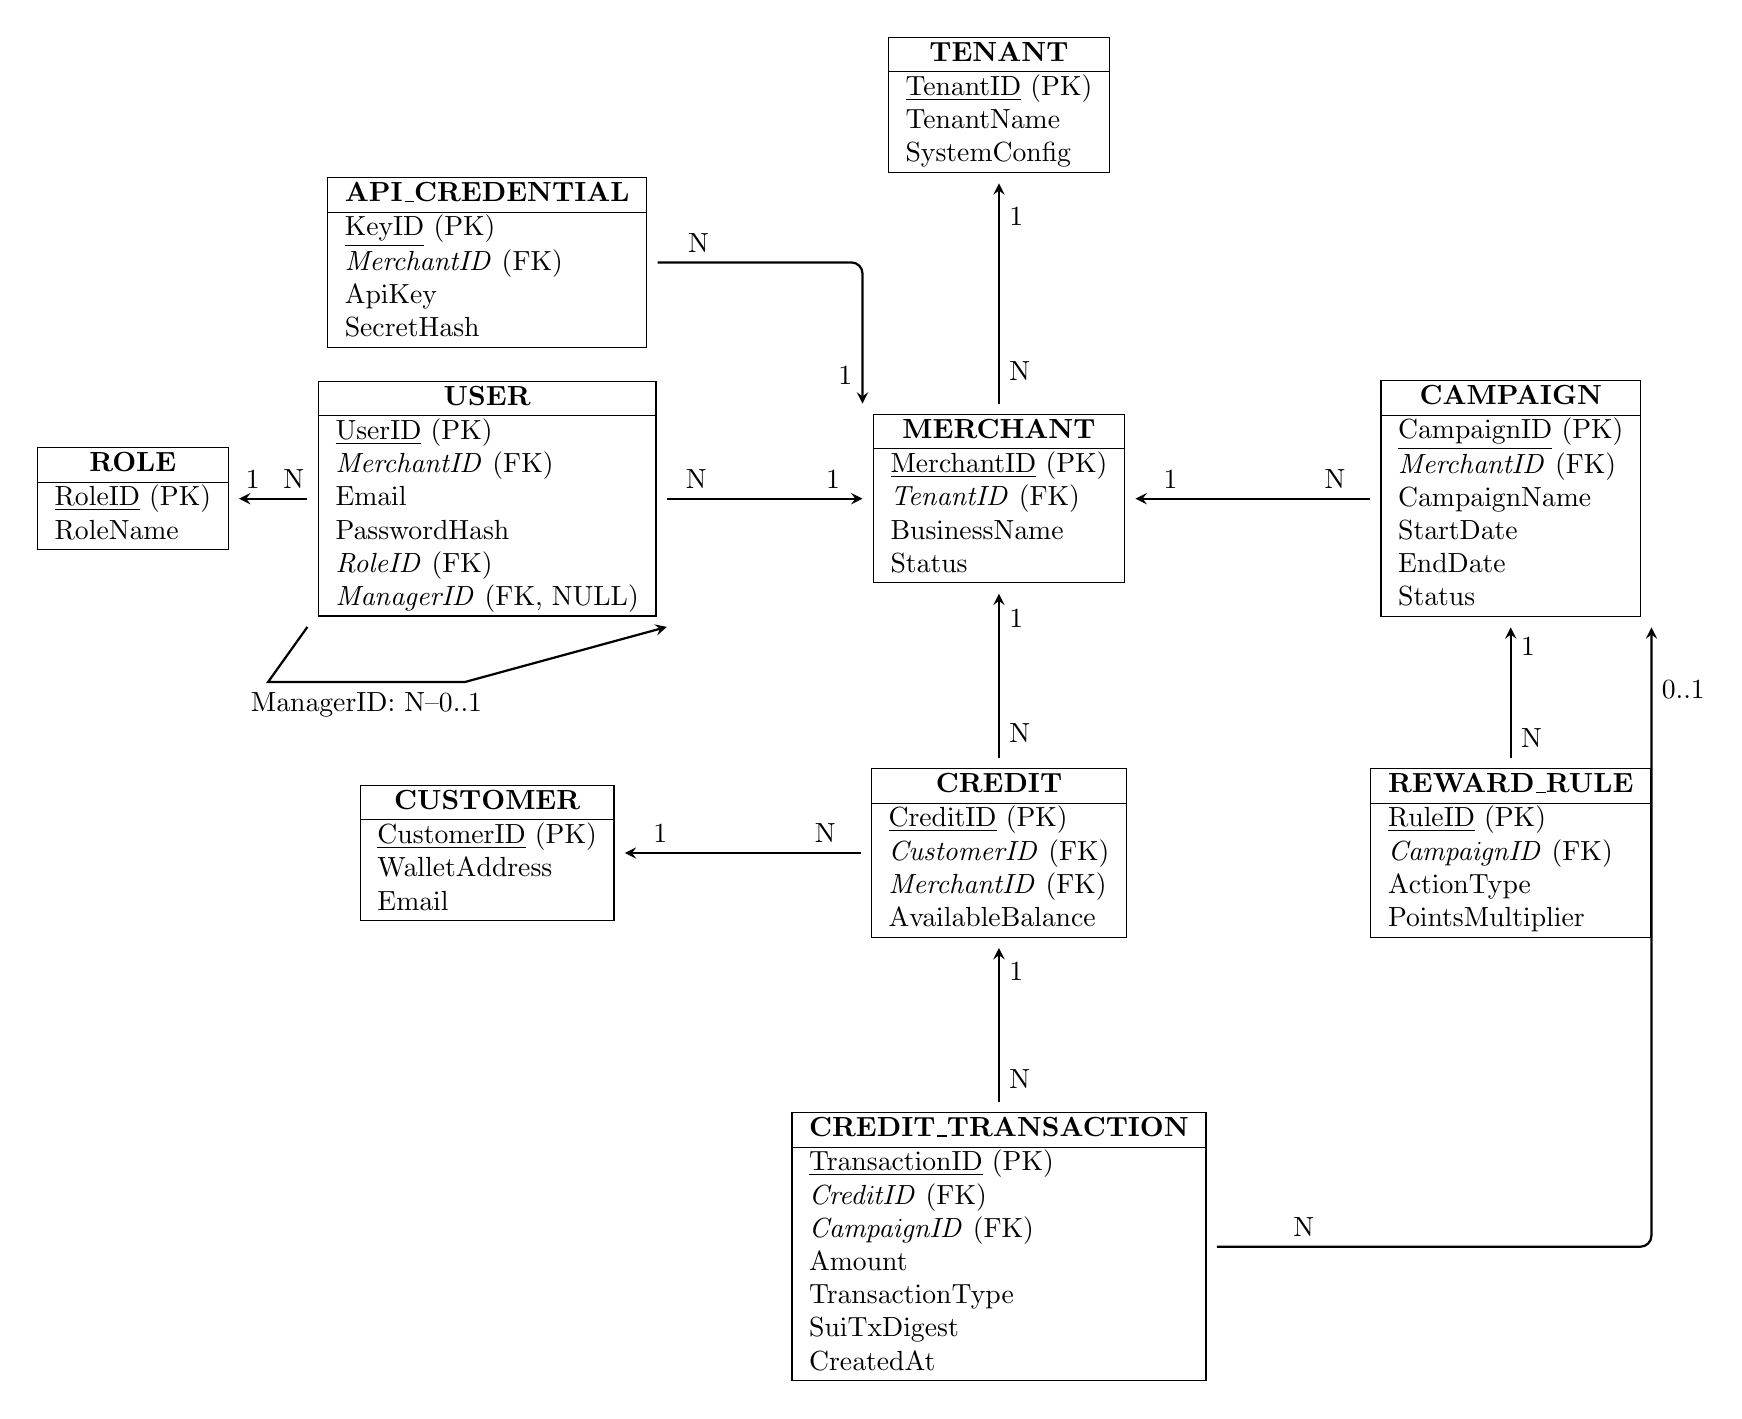
\begin{tikzpicture}[>=stealth, thick]

        % Bảng TENANT
        \node (tenant) at (0, 6.5) {
            \begin{tabular}{|l|}
            \hline
            \multicolumn{1}{|c|}{\textbf{TENANT}} \\ \hline
            \underline{TenantID} (PK) \\
            TenantName \\
            SystemConfig \\ \hline
            \end{tabular}
        };

        % Bảng MERCHANT
        \node (merchant) at (0, 1.5) {
            \begin{tabular}{|l|}
            \hline
            \multicolumn{1}{|c|}{\textbf{MERCHANT}} \\ \hline
            \underline{MerchantID} (PK) \\
            \textit{TenantID} (FK) \\
            BusinessName \\
            Status \\ \hline
            \end{tabular}
        };

        % Bảng API_CREDENTIAL (Đã bổ sung)
        \node (api) at (-6.5, 4.5) {
            \begin{tabular}{|l|}
            \hline
            \multicolumn{1}{|c|}{\textbf{API\_CREDENTIAL}} \\ \hline
            \underline{KeyID} (PK) \\
            \textit{MerchantID} (FK) \\
            ApiKey \\
            SecretHash \\ \hline
            \end{tabular}
        };

        % Bảng USER
        \node (user) at (-6.5, 1.5) {
            \begin{tabular}{|l|}
            \hline
            \multicolumn{1}{|c|}{\textbf{USER}} \\ \hline
            \underline{UserID} (PK) \\
            \textit{MerchantID} (FK) \\
            Email \\
            PasswordHash \\
            \textit{RoleID} (FK) \\
            \textit{ManagerID} (FK, NULL) \\ \hline
            \end{tabular}
        };

        % Bang ROLE va quan he quan ly tu tham chieu
        \node (role) at (-11, 1.5) {
            \begin{tabular}{|l|}
            \hline
            \multicolumn{1}{|c|}{\textbf{ROLE}} \\ \hline
            \underline{RoleID} (PK) \\
            RoleName \\ \hline
            \end{tabular}
        };
        \draw[->] (user.west) -- node[pos=0.2, above] {N} node[pos=0.8, above] {1} (role.east);
        \draw[->] (user.south west) -- ++(-0.5,-0.7) -- ++(2.5,0)
            node[midway, below] {ManagerID: N--0..1} -- (user.south east);

        % Bảng CAMPAIGN
        \node (campaign) at (6.5, 1.5) {
            \begin{tabular}{|l|}
            \hline
            \multicolumn{1}{|c|}{\textbf{CAMPAIGN}} \\ \hline
            \underline{CampaignID} (PK) \\
            \textit{MerchantID} (FK) \\
            CampaignName \\
            StartDate \\
            EndDate \\
            Status \\ \hline
            \end{tabular}
        };

        % Bảng CUSTOMER
        \node (customer) at (-6.5, -3) {
            \begin{tabular}{|l|}
            \hline
            \multicolumn{1}{|c|}{\textbf{CUSTOMER}} \\ \hline
            \underline{CustomerID} (PK) \\
            WalletAddress \\
            Email \\ \hline
            \end{tabular}
        };

        % Bảng CREDIT (Bảng trung gian giải quyết quan hệ N-N)
        \node (credit) at (0, -3) {
            \begin{tabular}{|l|}
            \hline
            \multicolumn{1}{|c|}{\textbf{CREDIT}} \\ \hline
            \underline{CreditID} (PK) \\
            \textit{CustomerID} (FK) \\
            \textit{MerchantID} (FK) \\
            AvailableBalance \\ \hline
            \end{tabular}
        };

        % Bảng REWARD_RULE
        \node (rule) at (6.5, -3) {
            \begin{tabular}{|l|}
            \hline
            \multicolumn{1}{|c|}{\textbf{REWARD\_RULE}} \\ \hline
            \underline{RuleID} (PK) \\
            \textit{CampaignID} (FK) \\
            ActionType \\
            PointsMultiplier \\ \hline
            \end{tabular}
        };

        % Bảng CREDIT_TRANSACTION
        \node (transaction) at (0, -8) {
            \begin{tabular}{|l|}
            \hline
            \multicolumn{1}{|c|}{\textbf{CREDIT\_TRANSACTION}} \\ \hline
            \underline{TransactionID} (PK) \\
            \textit{CreditID} (FK) \\
            \textit{CampaignID} (FK) \\
            Amount \\
            TransactionType \\
            SuiTxDigest \\
            CreatedAt \\ \hline
            \end{tabular}
        };

        % ========================================================
        % VẼ DÂY NỐI CÓ GẮN NHÃN BẢN SỐ (1 và N)
        % ========================================================
        
        % MERCHANT -> TENANT
        \draw[->] (merchant.north) -- node[pos=0.15, right] {N} node[pos=0.85, right] {1} (tenant.south);
        
        % API -> MERCHANT (Dây gấp khúc)
        \draw[->, rounded corners] (api.east) -| node[pos=0.1, above] {N} node[pos=0.9, left] {1} (merchant.north west);
        
        % USER -> MERCHANT
        \draw[->] (user.east) -- node[pos=0.15, above] {N} node[pos=0.85, above] {1} (merchant.west);
        
        % CAMPAIGN -> MERCHANT
        \draw[->] (campaign.west) -- node[pos=0.15, above] {N} node[pos=0.85, above] {1} (merchant.east);
        
        % CREDIT -> MERCHANT
        \draw[->] (credit.north) -- node[pos=0.15, right] {N} node[pos=0.85, right] {1} (merchant.south);
        
        % CREDIT -> CUSTOMER
        \draw[->] (credit.west) -- node[pos=0.15, above] {N} node[pos=0.85, above] {1} (customer.east);
        
        % REWARD_RULE -> CAMPAIGN
        \draw[->] (rule.north) -- node[pos=0.15, right] {N} node[pos=0.85, right] {1} (campaign.south);
        
        % TRANSACTION -> CREDIT
        \draw[->] (transaction.north) -- node[pos=0.15, right] {N} node[pos=0.85, right] {1} (credit.south);
        
        % TRANSACTION -> CAMPAIGN (Dây gấp khúc vòng lên)
        \draw[->, rounded corners] (transaction.east) -| node[pos=0.1, above] {N} node[pos=0.95, right] {0..1} (campaign.south east);

    \end{tikzpicture}
    }
    \caption{Sơ đồ Lược đồ Logic chi tiết hệ thống OctaPoint CaaS}
    \label{fig:sodo_logic_tikz}
\end{figure}

\textit{Ghi chú:} Sơ đồ thể hiện rõ việc phân rã mối kết hợp N-N giữa Khách hàng và Doanh nghiệp thông qua thực thể trung gian \texttt{CREDIT}. Các đường liên kết chỉ hướng tham chiếu từ Khóa ngoại (nhánh N) trỏ tới Khóa chính (nhánh 1), đảm bảo chặt chẽ ràng buộc toàn vẹn tham chiếu.
Mỗi cặp (CustomerID, MerchantID) ở CREDIT có tối đa một bản ghi. Nhãn N chỉ số lượng tối đa ở phía tham chiếu; RoleID bắt buộc, ManagerID và CampaignID của giao dịch tùy chọn.

\section{Từ điển Dữ liệu (Data Dictionary)}

Từ điển dữ liệu (Data Dictionary) mô tả chi tiết cấu trúc vật lý của các bảng trong cơ sở dữ liệu. Nó bao gồm tên các thuộc tính, kiểu dữ liệu, các ràng buộc toàn vẹn (Khóa chính - PK, Khóa ngoại - FK, Not Null) và diễn giải ý nghĩa của từng trường dữ liệu để chuẩn bị cho bước triển khai vật lý ở Chương 4.

\subsection{Bảng TENANT (Đơn vị thuê bao)}
Lưu trữ thông tin về các đơn vị khách hàng lớn thuê hệ thống OctaPoint CaaS.

\begin{table}[H]
    \centering
    \renewcommand{\arraystretch}{1.3}
    \begin{tabularx}{\textwidth}{|>{\raggedright\arraybackslash}p{3cm}|>{\raggedright\arraybackslash}p{2.8cm}|>{\raggedright\arraybackslash}p{2cm}|>{\raggedright\arraybackslash}X|}
        \hline
        \textbf{Tên thuộc tính} & \textbf{Kiểu dữ liệu} & \textbf{Ràng buộc} & \textbf{Mô tả} \\ \hline
        TenantID & VARCHAR(36) & PK, NOT NULL & Mã định danh duy nhất (UUID). \\ \hline
        TenantName & NVARCHAR(255) & NOT NULL & Tên định danh của đơn vị thuê bao. \\ \hline
        SystemConfig & NVARCHAR(MAX) & NULL, CHECK & Cấu hình hệ thống riêng của Tenant. \\ \hline
    \end{tabularx}
\end{table}

\subsection{Bảng MERCHANT (Doanh nghiệp đối tác)}
Lưu trữ thông tin các doanh nghiệp/cửa hàng trực thuộc một Tenant.

\begin{table}[H]
    \centering
    \renewcommand{\arraystretch}{1.3}
    \begin{tabularx}{\textwidth}{|>{\raggedright\arraybackslash}p{3cm}|>{\raggedright\arraybackslash}p{2.8cm}|>{\raggedright\arraybackslash}p{2cm}|>{\raggedright\arraybackslash}X|}
        \hline
        \textbf{Tên thuộc tính} & \textbf{Kiểu dữ liệu} & \textbf{Ràng buộc} & \textbf{Mô tả} \\ \hline
        MerchantID & VARCHAR(36) & PK, NOT NULL & Mã định danh duy nhất của Merchant. \\ \hline
        TenantID & VARCHAR(36) & FK, NOT NULL & Tham chiếu đến bảng TENANT. \\ \hline
        BusinessName & NVARCHAR(255) & NOT NULL & Tên thương hiệu/doanh nghiệp. \\ \hline
        Status & VARCHAR(20) & NOT NULL & Trạng thái hoạt động (Active, Suspended). \\ \hline
    \end{tabularx}
\end{table}

\subsection{Bảng USER (Tài khoản nhân sự)}
Quản lý tài khoản đăng nhập của nhân viên thuộc các Merchant.

\begin{table}[H]
    \centering
    \renewcommand{\arraystretch}{1.3}
    \begin{tabularx}{\textwidth}{|>{\raggedright\arraybackslash}p{3cm}|>{\raggedright\arraybackslash}p{2.8cm}|>{\raggedright\arraybackslash}p{2cm}|>{\raggedright\arraybackslash}X|}
        \hline
        \textbf{Tên thuộc tính} & \textbf{Kiểu dữ liệu} & \textbf{Ràng buộc} & \textbf{Mô tả} \\ \hline
        UserID & VARCHAR(36) & PK, NOT NULL & Mã định danh tài khoản. \\ \hline
        MerchantID & VARCHAR(36) & FK, NOT NULL & Tham chiếu đến bảng MERCHANT. \\ \hline
        Email & VARCHAR(255) & UNIQUE, NOT NULL & Email đăng nhập (duy nhất). \\ \hline
        PasswordHash & VARCHAR(255) & NOT NULL & Chuỗi băm mật khẩu bảo mật. \\ \hline
        RoleID & INT & FK, NOT NULL & Mã quyền hạn của người dùng. \\ \hline
        ManagerID & VARCHAR(36) & FK, NULL & Mã người quản lý trực tiếp (tham chiếu đến UserID). \\ \hline
    \end{tabularx}
\end{table}

\subsubsection{Bảng ROLE (Vai trò)}
Lưu trữ thông tin các nhóm quyền hạn để phân quyền người dùng trong hệ thống.

\begin{table}[H]
\centering
\begin{tabularx}{\textwidth}{|>{\raggedright\arraybackslash}p{3cm}|>{\raggedright\arraybackslash}p{2.8cm}|>{\raggedright\arraybackslash}p{2cm}|>{\raggedright\arraybackslash}X|}
\hline
\textbf{Tên thuộc tính} & \textbf{Kiểu dữ liệu} & \textbf{Ràng buộc} & \textbf{Mô tả} \\ \hline
RoleID & INT & PK, NOT NULL & Mã định danh vai trò. \\ \hline
RoleName & NVARCHAR(50) & NOT NULL & Tên hiển thị của vai trò (VD: Admin, Staff). \\ \hline
\end{tabularx}
\end{table}

\subsection{Bảng CUSTOMER (Khách hàng)}
Quản lý thông tin định danh của khách hàng tích điểm.

\begin{table}[H]
    \centering
    \renewcommand{\arraystretch}{1.3}
    \begin{tabularx}{\textwidth}{|>{\raggedright\arraybackslash}p{3cm}|>{\raggedright\arraybackslash}p{2.8cm}|>{\raggedright\arraybackslash}p{2cm}|>{\raggedright\arraybackslash}X|}
        \hline
        \textbf{Tên thuộc tính} & \textbf{Kiểu dữ liệu} & \textbf{Ràng buộc} & \textbf{Mô tả} \\ \hline
        CustomerID & VARCHAR(36) & PK, NOT NULL & Mã định danh khách hàng nội bộ. \\ \hline
        WalletAddress & VARCHAR(100) & UNIQUE*, NULL & Địa chỉ ví blockchain (Sui) dùng cho Walletless Auth. \\ \hline
        Email & VARCHAR(255) & NULL & Địa chỉ email (Định danh Web2). \\ \hline
    \end{tabularx}
\end{table}

\subsection{Bảng CAMPAIGN (Chiến dịch)}
Quản lý các chương trình khuyến mãi, tích/đổi điểm.

\begin{table}[H]
    \centering
    \renewcommand{\arraystretch}{1.3}
    \begin{tabularx}{\textwidth}{|>{\raggedright\arraybackslash}p{3cm}|>{\raggedright\arraybackslash}p{2.8cm}|>{\raggedright\arraybackslash}p{2cm}|>{\raggedright\arraybackslash}X|}
        \hline
        \textbf{Tên thuộc tính} & \textbf{Kiểu dữ liệu} & \textbf{Ràng buộc} & \textbf{Mô tả} \\ \hline
        CampaignID & VARCHAR(36) & PK, NOT NULL & Mã định danh chiến dịch. \\ \hline
        MerchantID & VARCHAR(36) & FK, NOT NULL & Tham chiếu đến bảng MERCHANT. \\ \hline
        CampaignName & NVARCHAR(255) & NOT NULL & Tên chiến dịch. \\ \hline
        StartDate & DATETIME & NOT NULL & Thời gian bắt đầu. \\ \hline
        EndDate & DATETIME & NULL & Thời điểm kết thúc (NULL nếu vô thời hạn). \\ \hline
        Status & VARCHAR(20) & NOT NULL & Trạng thái (Draft, Active, Expired). \\ \hline
    \end{tabularx}
\end{table}

\subsection{Bảng CREDIT\_TRANSACTION (Sổ cái giao dịch điểm)}
Lưu vết toàn bộ các giao dịch cộng/trừ điểm thưởng, có lưu băm trên blockchain.

\begin{table}[H]
    \centering
    \renewcommand{\arraystretch}{1.3}
    \begin{tabularx}{\textwidth}{|>{\raggedright\arraybackslash}p{3cm}|>{\raggedright\arraybackslash}p{2.8cm}|>{\raggedright\arraybackslash}p{2cm}|>{\raggedright\arraybackslash}X|}
        \hline
        \textbf{Tên thuộc tính} & \textbf{Kiểu dữ liệu} & \textbf{Ràng buộc} & \textbf{Mô tả} \\ \hline
        TransactionID & VARCHAR(36) & PK, NOT NULL & Mã giao dịch định danh. \\ \hline
        CreditID & VARCHAR(36) & FK, NOT NULL & Tham chiếu đến ví điểm. \\ \hline
        CampaignID & VARCHAR(36) & FK, NULL & Tham chiếu đến chiến dịch. \\ \hline
        Amount & DECIMAL(18,2) & NOT NULL & Biến động có dấu: Earn $>0$, Redeem $<0$, Refund khác 0. \\ \hline
        TransactionType & VARCHAR(50) & NOT NULL & Loại giao dịch (Earn, Redeem, Refund). \\ \hline
        SuiTxDigest & VARCHAR(100) & UNIQUE*, NULL & Mã băm giao dịch trên mạng lưới Sui. \\ \hline
        CreatedAt & DATETIME & NOT NULL & Thời gian phát sinh giao dịch. \\ \hline
    \end{tabularx}
\end{table}

\subsection{Bảng CREDIT}
\begin{table}[H]
\centering
\small
\begin{tabularx}{\textwidth}{|>{\raggedright\arraybackslash}p{3cm}|>{\raggedright\arraybackslash}p{2.8cm}|>{\raggedright\arraybackslash}p{2cm}|>{\raggedright\arraybackslash}X|}
\hline
Thuộc tính & Kiểu dữ liệu & Ràng buộc & Mô tả \\ \hline
CreditID & VARCHAR(36) & PK, NOT NULL & Định danh ví. \\ \hline
CustomerID & VARCHAR(36) & FK, NOT NULL & Tham chiếu CUSTOMER. \\ \hline
MerchantID & VARCHAR(36) & FK, NOT NULL & Tham chiếu MERCHANT. \\ \hline
AvailableBalance & DECIMAL(18,2) & NOT NULL, CHECK & Số dư không âm, mặc định 0. \\ \hline
\end{tabularx}
\end{table}
\subsection{Bảng REWARD\_RULE}
\begin{table}[H]
\centering
\small
\begin{tabularx}{\textwidth}{|>{\raggedright\arraybackslash}p{3cm}|>{\raggedright\arraybackslash}p{2.8cm}|>{\raggedright\arraybackslash}p{2cm}|>{\raggedright\arraybackslash}X|}
\hline
Thuộc tính & Kiểu dữ liệu & Ràng buộc & Mô tả \\ \hline
RuleID & VARCHAR(36) & PK, NOT NULL & Định danh quy tắc. \\ \hline
CampaignID & VARCHAR(36) & FK, NOT NULL & Tham chiếu CAMPAIGN. \\ \hline
ActionType & VARCHAR(50) & NOT NULL & Mã hành động mở rộng, ví dụ Purchase, Birthday. \\ \hline
PointsMultiplier & DECIMAL(5,2) & NOT NULL, CHECK & Hệ số lớn hơn 0. \\ \hline
\end{tabularx}
\end{table}
\subsection{Bảng API\_CREDENTIAL}
\begin{table}[H]
\centering
\small
\begin{tabularx}{\textwidth}{|>{\raggedright\arraybackslash}p{3cm}|>{\raggedright\arraybackslash}p{2.8cm}|>{\raggedright\arraybackslash}p{2cm}|>{\raggedright\arraybackslash}X|}
\hline
Thuộc tính & Kiểu dữ liệu & Ràng buộc & Mô tả \\ \hline
KeyID & VARCHAR(36) & PK, NOT NULL & Định danh bản ghi khóa. \\ \hline
MerchantID & VARCHAR(36) & FK, NOT NULL & Tham chiếu MERCHANT. \\ \hline
ApiKey & VARCHAR(255) & UNIQUE, NOT NULL & Mã khóa công khai duy nhất. \\ \hline
SecretHash & VARCHAR(255) & NOT NULL & Giá trị băm của secret. \\ \hline
\end{tabularx}
\end{table}

\textit{Ràng buộc bổ sung:} UNIQUE* nghĩa là duy nhất khi khác NULL, được triển khai bằng chỉ mục có điều kiện. CREDIT có UNIQUE(CustomerID, MerchantID). EndDate phải không trước StartDate khi có giá trị; các miền Status và TransactionType có CHECK. SystemConfig phải là JSON object/array hợp lệ khi khác NULL. CreatedAt mặc định GETDATE(). ManagerID tham chiếu USER và không bằng UserID của chính dòng. Nội dung đầy đủ nằm trong \texttt{database/schema.sql}.


\chapter{Thiết kế Vật lý và Triển khai}

Theo quy trình thiết kế cơ sở dữ liệu, thiết kế vật lý không làm thay đổi ý nghĩa dữ liệu mà quyết định cách Hệ quản trị CSDL (DBMS) lưu trữ, đọc, ghi và tìm kiếm dữ liệu tối ưu nhất dựa trên tải công việc (workload). 

Chương này sử dụng lược đồ logic đã chuẩn hóa và các đặc tả workload làm đầu vào, từ đó tiến hành lựa chọn tổ chức lưu trữ, đánh chỉ mục và xuất ra cấu trúc mã lệnh DDL vật lý.

\section{Đặc tả Workload và Chọn hệ quản trị}

\subsection{Đặc tả tải công việc}
Bảng \texttt{CREDIT\_TRANSACTION} nhận nhiều thao tác ghi khi khách hàng tích/tiêu điểm. Các truy vấn chính gồm tìm ví theo khách hàng và Merchant, xem lịch sử theo thời gian và thống kê theo chiến dịch. Đây là giả định thiết kế; chưa có số liệu tải thực tế để chứng minh độ trễ.

\subsection{Lựa chọn SQL Server}
Đồ án thống nhất sử dụng \textbf{Microsoft SQL Server 2016 trở lên}, ngôn ngữ \textbf{T-SQL}, phù hợp với DDL và truy vấn mẫu. Đề xuất sản phẩm gốc có lựa chọn hệ quản trị khác; bài môn học được tự chọn hệ quản trị nên sử dụng SQL Server và thống nhất cú pháp T-SQL trong toàn báo cáo.
\begin{itemize}
    \item Các bảng dùng rowstore với \texttt{PRIMARY KEY CLUSTERED} khai báo rõ trong DDL. Cấu trúc B+ tree hỗ trợ tìm theo khóa và khoảng trên khóa chỉ mục.
    \item Giao dịch SQL hỗ trợ tính ACID cho các thay đổi trong cơ sở dữ liệu. Tầng dịch vụ phải gói thao tác ghi lịch sử và cập nhật số dư trong cùng giao dịch, xử lý đồng thời và rollback khi lỗi.
    \item \texttt{NVARCHAR} lưu văn bản Unicode; \texttt{DECIMAL} lưu điểm chính xác theo hai chữ số thập phân; \texttt{NVARCHAR(MAX)} kèm \texttt{ISJSON} lưu cấu hình JSON.
\end{itemize}
Khóa UUID dạng \texttt{VARCHAR(36)} được giữ để đồng bộ với mô hình hiện có. UUID ngẫu nhiên có thể gây phân mảnh và tăng kích thước chỉ mục; cần đo đạc trước khi lựa chọn khóa cụm khác. Không có tổ chức lưu trữ nào bảo đảm hiệu năng tốt cho mọi workload. Giao dịch SQL không tự tạo tính nguyên tử xuyên SQL Server và blockchain Sui.

\section{Ánh xạ Kiểu dữ liệu và Ràng buộc}

\subsection{Kiểu dữ liệu trên SQL Server}
\begin{itemize}
    \item ID dùng \texttt{VARCHAR(36)} để lưu UUID do ứng dụng sinh; riêng \texttt{RoleID} dùng \texttt{INT}. UUID không thay thế kiểm soát truy cập.
    \item Tên hiển thị dùng \texttt{NVARCHAR}; email, mã khóa và mã băm dùng \texttt{VARCHAR}. Mật khẩu được băm, không lưu bản rõ.
    \item Số dư và biến động dùng \texttt{DECIMAL(18,2)}; hệ số dùng \texttt{DECIMAL(5,2)}. Thời điểm dùng \texttt{DATETIME} theo mô hình hiện tại.
    \item \texttt{SystemConfig} dùng \texttt{NVARCHAR(MAX)} nullable, kiểm tra JSON object/array bằng \texttt{ISJSON}; không sử dụng kiểu JSON riêng của hệ quản trị khác.
\end{itemize}

\subsection{Ràng buộc triển khai}
Mỗi bảng có PK; các FK dùng \texttt{ON DELETE NO ACTION}. \texttt{User.Email} duy nhất toàn hệ thống và không NULL; \texttt{ApiKey} cũng duy nhất và không NULL. Cặp \texttt{(CustomerID, MerchantID)} của CREDIT duy nhất.

\texttt{WalletAddress} và \texttt{SuiTxDigest} nullable dùng \texttt{UNIQUE INDEX ... WHERE ... IS NOT NULL}. UNIQUE thông thường trên một cột nullable của SQL Server chỉ cho phép tối đa một NULL, không phù hợp yêu cầu nhiều bản ghi chưa có định danh.

Các CHECK bảo đảm số dư không âm, hệ số dương, ngày kết thúc không trước ngày bắt đầu và miền trạng thái thống nhất. \texttt{Amount} là biến động có dấu: Earn dương, Redeem âm, Refund khác 0 và mang dấu đảo của giao dịch được hoàn. DDL chưa xác minh giao dịch gốc của Refund. \texttt{ActionType} là mã hành động mở rộng, không áp đặt danh sách đóng khi chưa có đặc tả đầy đủ.

FK tự tham chiếu của \texttt{ManagerID} kiểm tra người quản lý tồn tại; CHECK loại bỏ tự quản lý trực tiếp. Kiểm tra chu trình nhiều cấp và phạm vi Merchant thuộc tầng dịch vụ, chưa được DDL này bảo đảm.

\section{Chiến lược Đánh chỉ mục}

Chỉ mục giảm chi phí đọc ở một số truy vấn nhưng tăng dung lượng và chi phí ghi. Việc lựa chọn phải dựa trên bộ lọc, phép nối, thứ tự kết quả và số liệu thực thi.

\subsection{Chỉ mục triển khai}
\begin{itemize}
    \item Mọi PK được khai báo \texttt{CLUSTERED} trong \texttt{database/schema.sql}. UNIQUE tạo chỉ mục hỗ trợ các khóa nghiệp vụ; không tạo thêm chỉ mục Email trùng chức năng.
    \item SQL Server không tự tạo chỉ mục cho FK. DDL bổ sung chỉ mục cho TenantID của MERCHANT; MerchantID, RoleID, ManagerID của USER; MerchantID của API\_CREDENTIAL, CAMPAIGN, CREDIT; CampaignID của REWARD\_RULE và CREDIT\_TRANSACTION.
    \item CREDIT dùng UNIQUE \texttt{(CustomerID, MerchantID)}, đồng thời hỗ trợ tra cứu theo CustomerID ở cột dẫn đầu.
    \item Chỉ mục \texttt{(CreditID, CreatedAt DESC)} hỗ trợ lọc lịch sử một ví theo thời gian. Không tạo riêng chỉ mục CreditID trùng tiền tố.
    \item Hai chỉ mục duy nhất có điều kiện bảo vệ WalletAddress và SuiTxDigest khi khác NULL.
\end{itemize}

\subsection{Đánh giá và giới hạn}
Tỷ lệ $NDV(A)/|R|$ biểu diễn mức phân biệt giá trị, không phải tỷ lệ dòng thỏa một điều kiện cụ thể. Hiệu quả chỉ mục còn phụ thuộc phân bố dữ liệu, số dòng trả về và chi phí truy cập.

Chưa tạo chỉ mục đơn trên Status (Merchant: Active/Suspended; Campaign: Draft/Active/Expired) hoặc TransactionType (Earn/Redeem/Refund). Miền giá trị nhỏ không có nghĩa chỉ mục luôn vô ích: chỉ mục ghép hoặc có điều kiện vẫn có thể hữu ích với workload phù hợp. Cần kiểm tra execution plan, statistics và chi phí ghi trước khi bổ sung.

\section{Mã lệnh tạo bảng (DDL - Data Definition Language)}

Mã nguồn chuẩn nằm tại \texttt{database/schema.sql}, dùng SQL Server 2016 trở lên và chạy một lần trên cơ sở dữ liệu trống với schema mặc định \texttt{dbo}. Báo cáo nạp trực tiếp file này để tránh sai lệch giữa mã thực thi và nội dung trình bày. Đây là script khởi tạo, không phải migration cho cơ sở dữ liệu đã có dữ liệu.

\lstinputlisting[style=sqlstyle]{database/schema.sql}

Các khóa ngoại sử dụng \texttt{ON DELETE NO ACTION}. Chỉ mục duy nhất có điều kiện cho phép nhiều giá trị NULL ở \texttt{WalletAddress} và \texttt{SuiTxDigest}, nhưng ngăn trùng giá trị đã được cung cấp.

\textbf{Giới hạn triển khai:} Script triển khai cấu trúc, khóa, miền giá trị và chỉ mục. Script chưa triển khai phân quyền ghi sổ cái, tự động cập nhật số dư, kiểm tra chu trình quản lý, kiểm tra liên kết cùng Merchant hay cơ chế đồng bộ blockchain. Các yêu cầu này được nêu rõ ở Chương 1 và cần triển khai tại tầng dịch vụ/quyền truy cập trước khi vận hành.

\section{Tối ưu hóa truy xuất dữ liệu}

Dựa trên pipeline xử lý truy vấn của hệ quản trị CSDL, việc viết câu lệnh SQL là chưa đủ. Hệ thống cần tối ưu hóa cây truy vấn (Query Tree) thông qua các luật biến đổi tương đương để giảm thiểu chi phí bộ nhớ và I/O trước khi lập kế hoạch thực thi (Execution Plan).

\subsection{Bài toán truy vấn}
\textbf{Yêu cầu:} Lấy ra Mã giao dịch (\texttt{TransactionID}) và Số điểm (\texttt{Amount}) của các giao dịch cộng điểm lớn hơn 500, thuộc về các Chiến dịch (\texttt{CAMPAIGN}) đang ở trạng thái hoạt động (\texttt{'Active'}).

\textbf{Biểu thức đại số quan hệ:}
\[
\begin{aligned}
T' &= \sigma_{Amount > 500 \,\wedge\, TransactionType = \text{'Earn'}}(T),\\
C' &= \sigma_{Status = \text{'Active'}}(C),\\
Q &= \pi_{TransactionID,Amount}(T' \bowtie_{T'.CampaignID=C'.CampaignID} C').
\end{aligned}
\]
Trong đó $T$ là CREDIT\_TRANSACTION, $C$ là CAMPAIGN. Phép nối dùng điều kiện bằng CampaignID, không phải nối tự nhiên trên tất cả thuộc tính cùng tên.

\subsection{Cây truy vấn trước và sau khi tối ưu}

Theo luật biến đổi tương đương, phép chọn (Selection - $\sigma$) nếu được đẩy xuống trước phép kết nối (Join - $\bowtie$) sẽ giúp giảm thiểu đáng kể kích thước dữ liệu trung gian.

\begin{figure}[H]
    \centering
    \resizebox{\textwidth}{!}{ % Ép toàn bộ sơ đồ tự động co lại vừa khít 100% chiều ngang trang giấy
    \begin{tikzpicture}[
        box/.style={rectangle, draw=black, rounded corners, inner sep=12pt, text centered, font=\normalsize},
        leaf/.style={rectangle, draw=black, inner sep=10pt, text centered, font=\normalsize\bfseries}
    ]
        % ================= CÂY CHƯA TỐI ƯU =================
        \node[font=\Large\bfseries] at (0, 8.5) {Chưa tối ưu};
        
        \node[box] (proj1) at (0, 7) {$\pi_{TransactionID, Amount}$};
        \node[box] (sel1) at (0, 5) {$\sigma_{Amount > 500 \wedge TransactionType = \text{'Earn'} \wedge Status = \text{'Active'}}$};
        \node[box] (join1) at (0, 3) {$\bowtie_{CampaignID}$};
        
        \node[leaf] (trans1) at (-4.5, 0) {CREDIT\_TRANSACTION};
        \node[leaf] (camp1) at (4.5, 0) {CAMPAIGN};
        
        \draw[->, thick] (sel1) -- (proj1);
        \draw[->, thick] (join1) -- (sel1);
        \draw[->, thick] (trans1) -- (join1);
        \draw[->, thick] (camp1) -- (join1);

        % ================= CÂY ĐÃ TỐI ƯU =================
        \node[font=\Large\bfseries] at (18, 8.5) {Đã đẩy phép chọn};
        
        \node[box] (proj2) at (18, 7) {$\pi_{TransactionID, Amount}$};
        \node[box] (join2) at (18, 5) {$\bowtie_{CampaignID}$};
        
        \node[box] (sel2_trans) at (13, 2.5) {$\sigma_{Amount > 500 \wedge TransactionType = \text{'Earn'}}$};
        \node[box] (sel2_camp) at (23, 2.5) {$\sigma_{Status = \text{'Active'}}$};
        
        \node[leaf] (trans2) at (13, 0) {CREDIT\_TRANSACTION};
        \node[leaf] (camp2) at (23, 0) {CAMPAIGN};
        
        \draw[->, thick] (join2) -- (proj2);
        \draw[->, thick] (sel2_trans) -- (join2);
        \draw[->, thick] (sel2_camp) -- (join2);
        \draw[->, thick] (trans2) -- (sel2_trans);
        \draw[->, thick] (camp2) -- (sel2_camp);
        
        % Đường phân cách dọc ở giữa
        \draw[dashed, thick, gray] (9, -1) -- (9, 9.5);
    \end{tikzpicture}
    }
    \caption{Cây truy vấn trước và sau khi tối ưu hóa bằng luật phân rã}
\end{figure}

\subsection{Câu lệnh SQL tương ứng}
\begin{lstlisting}[style=sqlstyle]
SELECT ct.TransactionID, ct.Amount
FROM CREDIT_TRANSACTION AS ct
JOIN CAMPAIGN AS c ON c.CampaignID = ct.CampaignID
WHERE ct.Amount > 500
  AND ct.TransactionType = 'Earn'
  AND c.Status = 'Active';
\end{lstlisting}

\subsection{Đánh giá thuật toán kết nối}
Đẩy phép chọn xuống có thể giảm số dòng trung gian; mức giảm thực tế phụ thuộc phân bố dữ liệu. SQL Server chọn Nested Loops, Hash hoặc Merge Join theo statistics, chỉ mục và chi phí ước lượng. Nested Loops thường phù hợp khi đầu vào ngoài nhỏ và phía trong có đường tra cứu hiệu quả; không thể kết luận chỉ từ việc CAMPAIGN nhỏ.

Đồ án chưa có execution plan hoặc số đo I/O, thời gian trước/sau. Vì vậy đây là phân tích biến đổi logic, không phải bằng chứng một thuật toán luôn được chọn hay truy vấn đã đạt mục tiêu hiệu năng.

\section{Một số câu truy vấn mẫu}

Dưới đây là các câu truy vấn T-SQL tiêu biểu để kiểm chứng thiết kế cơ sở dữ liệu trên hệ quản trị SQL Server.

\subsection{Truy vấn 1: Xem lịch sử giao dịch điểm của một khách hàng tại một cửa hàng}
\begin{lstlisting}[style=sqlstyle]
SELECT 
    ct.TransactionID,
    ct.TransactionType,
    ct.Amount,
    ct.CreatedAt
FROM CREDIT_TRANSACTION ct
JOIN CREDIT c ON ct.CreditID = c.CreditID
WHERE c.CustomerID = 'CUST_UUID_001'
  AND c.MerchantID = 'MERCH_UUID_002'
ORDER BY ct.CreatedAt DESC, ct.TransactionID DESC;
\end{lstlisting}

\subsection{Truy vấn 2: Tra cứu số dư điểm hiện tại của khách hàng tại các cửa hàng đang hoạt động}
\begin{lstlisting}[style=sqlstyle]
SELECT 
    m.BusinessName,
    c.AvailableBalance
FROM CREDIT c
JOIN MERCHANT m ON c.MerchantID = m.MerchantID
WHERE c.CustomerID = 'CUST_UUID_001'
  AND m.Status = 'Active'
ORDER BY c.AvailableBalance DESC, c.MerchantID;
\end{lstlisting}

\subsection{Truy vấn 3: Thống kê tổng số điểm đã phát hành theo từng chiến dịch có phát sinh tích điểm trong tháng hiện tại}
\begin{lstlisting}[style=sqlstyle]
DECLARE @MonthStart DATETIME = DATEFROMPARTS(YEAR(GETDATE()), MONTH(GETDATE()), 1);

SELECT 
    camp.CampaignName,
    COUNT(ct.TransactionID) AS TotalTransactions,
    SUM(ct.Amount) AS TotalPointsIssued
FROM CREDIT_TRANSACTION ct
JOIN CAMPAIGN camp ON ct.CampaignID = camp.CampaignID
WHERE camp.MerchantID = 'MERCH_UUID_002'
  AND ct.TransactionType = 'Earn'
  AND ct.CreatedAt >= @MonthStart
  AND ct.CreatedAt < DATEADD(MONTH, 1, @MonthStart)
GROUP BY camp.CampaignID, camp.CampaignName;
\end{lstlisting}
Khoảng thời gian nửa kín ở truy vấn 3 giữ cột CreatedAt nguyên dạng để bộ tối ưu có thể tận dụng chỉ mục phù hợp. Truy vấn hiện có chưa bảo đảm kế hoạch seek; cần kiểm tra execution plan.

Tổng điểm phát hành ở truy vấn 3 chỉ cộng giao dịch Earn, chưa trừ các giao dịch hoàn trả. Chiến dịch không có Earn trong tháng không xuất hiện do sử dụng INNER JOIN. Các mã khách hàng và cửa hàng trong ví dụ cần được thay bằng mã tồn tại trong dữ liệu thử.



\end{document}
